\documentclass{article} % A4 paper and 11pt font size
\setcounter{secnumdepth}{0}

\usepackage{amssymb, amsmath, amsfonts}
\usepackage{moreverb}
\usepackage{graphicx}
\usepackage{enumerate}
\usepackage{graphics}
\usepackage[margin=1.25in]{geometry}
\usepackage{color}
\usepackage{tocloft}
\renewcommand{\cftsecleader}{\cftdotfill{\cftdotsep}}
\usepackage{array}
\usepackage{float}
\usepackage{hyperref}
\usepackage{textcomp}
\usepackage[makeroom]{cancel}
\usepackage{bbold}
\usepackage{alltt}
\usepackage{physics}
\usepackage{mathtools}
\usepackage[normalem]{ulem}
\usepackage{amsthm}
\usepackage{tikz}
\usetikzlibrary{positioning}
\usetikzlibrary{arrows}
\usepackage{pgfplots}
\usepackage{bigints}
\allowdisplaybreaks
\pgfplotsset{compat=1.12}

\theoremstyle{plain}
\newtheorem*{theorem*}{Theorem}
\newtheorem{theorem}{Theorem}
\newtheorem*{lemma*}{Lemma}
\newtheorem{lemma}{Lemma}

\makeatletter
\newcommand{\BIGG}{\bBigg@{3}}
\newcommand{\vast}{\bBigg@{4}}
\newcommand{\Vast}{\bBigg@{5}}
\makeatother

\newenvironment{definition}[1][Definition]{\begin{trivlist}
\item[\hskip \labelsep {\bfseries #1}]}{\end{trivlist}}

\newcommand{\dy}{\partial_y}
\newcommand{\dyy}{\partial_{yy}}
\newcommand{\dxx}{\partial_{xx}}
\newcommand{\dxy}{\partial_{xy}}
\newcommand{\dyyy}{\partial_{yyy}}
\newcommand{\dxxx}{\partial_{xxx}}
\newcommand{\dx}{\partial_x}
\newcommand{\E}{\varepsilon}
\def\Rl{\mathbb{R}}
\def\Cx{\mathbb{C}}

\newcommand{\Ei}{\text{Ei}}

\usepackage[T1]{fontenc} % Use 8-bit encoding that has 256 glyphs
\usepackage{fourier} % Use the Adobe Utopia font for the document - comment this line to return to the LaTeX default
\usepackage[english]{babel} % English language/hyphenation

\usepackage{sectsty} % Allows customizing section commands
\allsectionsfont{\centering \normalfont\scshape} % Make all sections centered, the default font and small caps

\usepackage{fancyhdr} % Custom headers and footers
\pagestyle{fancy} % Makes all pages in the document conform to the custom headers and footers
\fancyhead[L]{\bf Sam Fleischer}
\fancyhead[C]{\bf UC Davis \\ Applied Mathematics (MAT207C)} % No page header - if you want one, create it in the same way as the footers below
\fancyhead[R]{\bf Spring 2016}

\fancyfoot[L]{\bf } % Empty left footer
\fancyfoot[C]{\bf \thepage} % Empty center footer
\fancyfoot[R]{\bf } % Page numbering for right footer
\renewcommand{\headrulewidth}{0pt} % Remove header underlines
\renewcommand{\footrulewidth}{0pt} % Remove footer underlines
\setlength{\headheight}{25pt} % Customize the height of the header

\newcommand{\VEC}[2]{\left\langle #1, #2 \right\rangle}
\newcommand{\ran}{\text{\rm ran }}
\newcommand{\Hilb}{\mathcal{H}}
\newcommand{\lap}{\Delta}

\newcommand{\littleo}[1]{\text{\scriptsize$\mathcal{O}$}\qty(#1)}

\DeclareMathOperator*{\esssup}{\text{ess~sup}}

\newcommand{\problem}[2]{
\vspace{.375cm}
\boxed{\begin{minipage}{\textwidth}
    \section{\bf #1}
    #2
\end{minipage}}
}

\numberwithin{equation}{section} % Number equations within sections (i.e. 1.1, 1.2, 2.1, 2.2 instead of 1, 2, 3, 4)
\numberwithin{figure}{section} % Number figures within sections (i.e. 1.1, 1.2, 2.1, 2.2 instead of 1, 2, 3, 4)
\numberwithin{table}{section} % Number tables within sections (i.e. 1.1, 1.2, 2.1, 2.2 instead of 1, 2, 3, 4)

\setlength\parindent{0pt} % Removes all indentation from paragraphs - comment this line for an assignment with lots of text

\newcommand{\horrule}[1]{\rule{\linewidth}{#1}} % Create horizontal rule command with 1 argument of height

\usepackage{xcolor}
\definecolor{light-gray}{gray}{0.9}

\title{ 
\normalfont \normalsize 
\textsc{UC Davis, Applied Mathematics (MAT207C), Spring 2016} \\ [25pt] % Your university, school and/or department name(s)
\horrule{2pt} \\[0.4cm] % Thin top horizontal rule
\Huge Homework \#7 \\ % The assignment title
\horrule{2pt} \\[0.5cm] % Thick bottom horizontal rule
}

\author{\huge Sam Fleischer} % Your name

\date{May 27, 2016} % Today's date or a custom date

\begin{document}\thispagestyle{empty}

\maketitle % Print the title

\makeatletter
\@starttoc{toc}
\makeatother

\pagebreak

%%%%%%%%%%%%%%%%%%%%%%%%%%%%%%%%%%%%%%
\problem{Problem 1}{Consider a one-dimensional layered medium with a periodic substructure of alternate layers of material one with thickness $\E\phi_1$ and diffusion coefficient $D_1$ and material two with thickness $\E\phi_2$ and diffusion coefficient $D_2$.  WIthout loss of generality take $\phi_2 = 1 - \phi_1$ so that $\phi_i$ represents the volume fraction of material $i$ and the length of the periodic cell is $\E$.

The steady-state diffusion equation is $$\dx\qty(D(x)\dx u) = f(x),$$ where $D(x) = D_i$ in material $i$.  Let $x_*$ represent a point on the interface between two layers.  At such points we require
\begin{align*}
    \lim_{x \rightarrow x_*^-} u(x) &= \lim_{x \rightarrow x_*^+} u(x) \\
    \lim_{x \rightarrow x_*^-} D_{u_x} &= \lim_{x \rightarrow x_*^+} D_{u_x},
\end{align*}
which enforce continuity of the solution and continuity of the flux.  Derive a homogenized steady-state diffusion equation.}
\begin{proof}
    First let $y = \frac{x}{\E}$.  Without loss of generality, rescale our equations such that the periodic structure has boundaries at each integer.  Then
    \begin{align*}
        D(y) = \begin{cases}
            D_1, & \text{ if } y \in (0, \phi) \\
            D_2, & \text{ if } y \in (\phi, 1).
        \end{cases}
    \end{align*}
    Next let $u(x) = v(x,y) = v_0(x,y) + v_1(x,y) + \dots$.  Then $$\dx u = \qty(\dx + \frac{1}{\E}\dy) v,$$ which shows
    \begin{align*}
        \qty(\dx + \frac{1}{\E}\dy)\qty(D(y)\qty(\dx + \frac{1}{\E}\dy)\qty(v_0 + \E v_1 + \dots)) = f(x).
    \end{align*}
    The highest order is $\frac{1}{\E^2}$, and the $\order{\frac{1}{\E^2}}$ equation is
    \begin{align*}
        &\dy\qty(D(y)\dy v_0) = 0 \\
        \implies &\begin{cases}
            \dy\qty(D_1\dy v_0) = 0, & \text{ if } y \in (0, \phi) \\
            \dy\qty(D_2\dy v_0) = 0, & \text{ if } y \in (\phi, 1)
        \end{cases} \\
        \implies v_0(x,y) &= \begin{cases}
            a_1(x) + b_1(x)y, & \text{ if } y \in (0, \phi) \\
            a_2(x) + b_2(x)y, & \text{ if } y \in (\phi, 1).
        \end{cases}
    \end{align*}
    Continuity of the solution and of the flux imply
    \begin{align*}
        \underbrace{\begin{cases}
                    a_1(x) + b_1(x)\phi = a_2(x) + b_2(x)\phi \\
                    a_1(x) = a_2(x) + b_2(x)
                \end{cases}}_{\text{continuity of the solution}} \qquad \text{and} \qquad \underbrace{\begin{cases}
                    D_1 b_1(x) = D_2 b_2(x).
                \end{cases}}_{\text{continuity of the flux}}
    \end{align*}
    Continuity of the solution shows us $$b_1(x) = \frac{\phi - 1}{\phi}b_2(x),$$ and thus
    \begin{align*}
        \qty[D_1\frac{\phi - 1}{\phi} - D_2]b_2(x) = 0 \qquad \implies \qquad b_2(x) = 0 \qquad \implies \qquad b_1(x) = 0 \qquad \implies \qquad a_1(x) = a_2(x)
    \end{align*}
    since $D_1,D_2 > 0$ and $\phi < 1$.  After defining $a(x) \coloneqq a_1(x) = a_2(x)$, we get $v_0(x,y) = a(x)$, which shows $\dy v_0 = 0$, $\dx v_0 = a'(x)$, and $\dxx v_0 = a''(x)$.  The $\order{\frac{1}{\E}}$ equation is
    \begin{align*}
        \cancelto{0}{\dx\qty(D(y)\dy v_0)} + \dy\qty(D(y)\dx v_0) + \dy(D(y)\dy v_1) = 0 \\
        \begin{cases}
            D_1 \qty(\cancelto{0}{\dy a'(x)} + \dyy v_1) = 0, & \text{ if } y \in (0, \phi) \\
            D_2 \qty(\cancelto{0}{\dy a'(x)} + \dyy v_1) = 0, & \text{ if } y \in (\phi, 1)
        \end{cases} \\
        \implies v_1(x,y) = \begin{cases}
            c_1(x) + d_1(x) y, & \text{ if } y \in (0, \phi) \\
            c_2(x) + d_2(x) y, & \text{ if } y \in (\phi, 1).
        \end{cases}
    \end{align*}
    Continuity of the solution and of the flux imply
    \begin{align*}
        \underbrace{\begin{cases}
                    c_1(x) + d_1(x)\phi = c_2(x) + d_2(x)\phi \\
                    c_1(x) = c_2(x) + d_2(x)
                \end{cases}}_{\text{continuity of the solution}} \qquad \text{and} \qquad \underbrace{\begin{cases}
                    D_1[a'(x) + d_1(x)] = D_2[a'(x) + d_2(x)].
                \end{cases}}_{\text{continuity of the flux}}
    \end{align*}
    Continuity of the solution shows us
    \begin{align*}
        d_1(x) = \frac{\phi - 1}{\phi}d_2(x),
    \end{align*}
    and thus
    \begin{align*}
        D_1\qty[a'(x) + \frac{\phi - 1}{\phi}d_2(x)] = D_2\qty[a'(x) + d_2(x)] \\
        \implies \qquad d_2(x) = \frac{\phi\qty(D_2 - D_1)a'(x)}{\qty(D_1 - D_2)\phi - D_1} \qquad \implies \qquad d_1(x) = \frac{\qty(\phi - 1) \qty(D_2 - D_1)a'(x)}{\qty(D_1 - D_2)\phi - D_1}.
    \end{align*}
    Finally, the $\order{1}$ equation is
    \begin{align*}
        \dx\qty(D(y)\dx v_0) + \dx\qty(D(y)\dy v_1) + \dy\qty(D(y) \dx v_1) + \dy\qty(D(y)\dy v_2) = f(x) \\
        \implies \int_0^1 D(y) \qty(a''(x) + \dxy v_1(x,y)) \dd y + \cancelto{0}{\underbrace{D(y)\qty[\dx v_1(x,y) + \dy v_2(x,y)]\bigg|_{y=0}^{y=1}}_{\text{cancels due to periodicity in $y$}}} = f(x) \\
        \implies D_1 a''(x)\int_0^\phi \dd y + D_2 a''(x)\int_\phi^1 \dd y + D_1d_1'(x)\int_0^\phi \dd y + D_2d_2'(x)\int_\phi^1 \dd y = f(x) \\
        \implies D_1\qty(a''(x) + d_1'(x))\phi + D_2\qty(a''(x) + d_2'(x))(1 - \phi) = f(x).
    \end{align*}
    Since $$d_1''(x) = \frac{(\phi - 1)(D_2 - D_1)}{(D_1 - D_2)\phi - D_1}a''(x) \qquad \text{and} \qquad d_2''(x) = \frac{\phi(D_2 - D_1)}{(D_1 - D_2)\phi - D_1}a''(x),$$
    then
    \begin{align*}
        D^*(x) \coloneqq \frac{a''(x)D_1D_2}{D_1(1 - \phi) + D_2\phi} = f(x).
    \end{align*}
    Finally, the homogenized equation is
    \begin{align*}
        \boxed{\dx\qty(D^*(x)\dx u) = f(x)}
    \end{align*}
\end{proof}







\problem{Problem 2}{Express the below equation in the standard in the standard form to apply the averaging theorem $\qty(\dot{\textbf{x}} = \E\textbf{f}\qty(\textbf{x},t), \textbf{f} \text{ periodic in time}),$ and give the averaged equations. $$\ddot{u} + 4\E\qty(\cos^2t)\dot{u} + u = 0.$$  Generate a numerical solution to the time-averaged equations and compare it with the solution of $$\ddot{v} + 2\E\dot{v} + v = 0,$$ in which the coefficient has been replaced with the time-averaged value without invoking the averaging theorem.}
\begin{proof}
    Let $\E \rightarrow 0$.  Thus $\ddot{u} + u = 0$.  This has the solution $u(t) = a(t)\cos(t + \phi(t))$, where $a$ and $\phi$ are parameters based on the small timescale.  Define $u_1 = u$ and $u_2 = \dot{u}$ (this is the derivative with respect to the long timescale.  Then
    \begin{align*}
        u_1 &= a(t)\cos(t + \phi(t)), \\
        u_2 &= -a(t)\sin(t + \phi(t)),
    \end{align*}
    and thus
    \begin{align*}
        a'(t)\cos(t + \phi(t)) - a(t)\sin(t + \phi(t))\qty(\phi'(t) + 1) = \dot{u_1} &= u_2 = -a(t)\sin(t + \phi(t)), \\
        -a'(t)\sin(t + \phi(t)) - a(t)\cos(t + \phi(t))\qty(\phi'(t) + 1) = \dot{u_2} &= -4\E\qty(\cos^2(t))u_1 - u_2 = -4\E\cos^2(t)\qty[-a(t)\sin(t + \phi(t))] - a(t)\cos(t + \phi(t)).
    \end{align*}
    We can solve for $a'(t)$ and $\phi'(t)$:
    \begin{align*}
        a'(t) &= -4\E\cos^2(t)\sin^2(t + \phi(t)), \\
        \phi'(t) &= -4\E\cos^2(t)\sin(t + \phi(t))\cos(t + \phi(t)).
    \end{align*}
    This is of the form $\dot{\textbf{x}} = \E\textbf{f}(\textbf{x},t)$ with $\textbf{f}$ periodic in $t$, and we can thus employ the averaging theorem:
    \begin{align*}
        \overline{a}'(t) &= \lim_{t \rightarrow \infty}\frac{1}{2t}\int_{-t}^t a'(t) \dd t \\
        \overline{\phi}'(t) &= \lim_{t \rightarrow \infty}\frac{1}{2t}\int_{-t}^t \phi'(t) \dd t.
    \end{align*}
    We calculate these integrals:
    \begin{align*}
        \overline{a}'(t) &= \E\lim_{t\rightarrow \infty}\frac{1}{2t}\qty[\qty(t + \sin(2t) + \frac{1}{4}\sin(4t))\cos(2\overline{\phi}(t)) - 2t - \sin(2t)] \\
        &= \E\lim_{t\rightarrow \infty}\qty[\qty(\frac{1}{2} + \cancelto{0}{\frac{\sin(2t) + \frac{1}{4}\sin(4t)}{2t}})\cos(2\overline{\phi}(t)) - 1 - \cancelto{0}{\frac{\sin(2t)}{2t}}] \\
        &= \E\qty[\frac{1}{2}\cos(2\overline{\phi}(t)) - 1] \\
        \overline{\phi}'(t) &= \E\lim_{t\rightarrow \infty} \frac{1}{2t}\qty[-\frac{1}{4}\qty(4t + 4\sin(2t) + \sin(4t))\sin(2\overline{\phi}(t))] \\
        &= \E\lim_{t\rightarrow\infty}\qty[\qty(-\frac{1}{2} - \cancelto{0}{\frac{\sin(2t)\frac{1}{4}\sin(4t)}{2t}})\sin(2\overline{\phi}(t))] \\
        &= -\E\frac{1}{2}\sin(2\overline{\phi}(t))
    \end{align*}
    and thus the averaged system is
    \begin{align*}
        \boxed{\qty[\begin{array}{c}\overline{a} \\ \overline{\phi}\end{array}]' = \E\qty[\begin{array}{c}\frac{1}{2}\cos(2\overline{\phi}(t)) - 1 \\ -\frac{1}{2}\sin(2\overline{\phi}(t))\end{array}]}
    \end{align*}
    We can solve this system numerically and plot the solution $u = \overline{a}\cos(t + \overline{\phi})$, as seen in the figure.  For reference, we also solve the system $\ddot{v} + 2\E\dot{v} + v = 0$ with initial condition $v(0) = 1$ and $v'(0) = 0$:
    \begin{align*}
        v(t) = e^{-\E t}\cos(\qty(\sqrt{1 - \E^2})t)
    \end{align*}

    \begin{figure}[ht!]
        \centering
        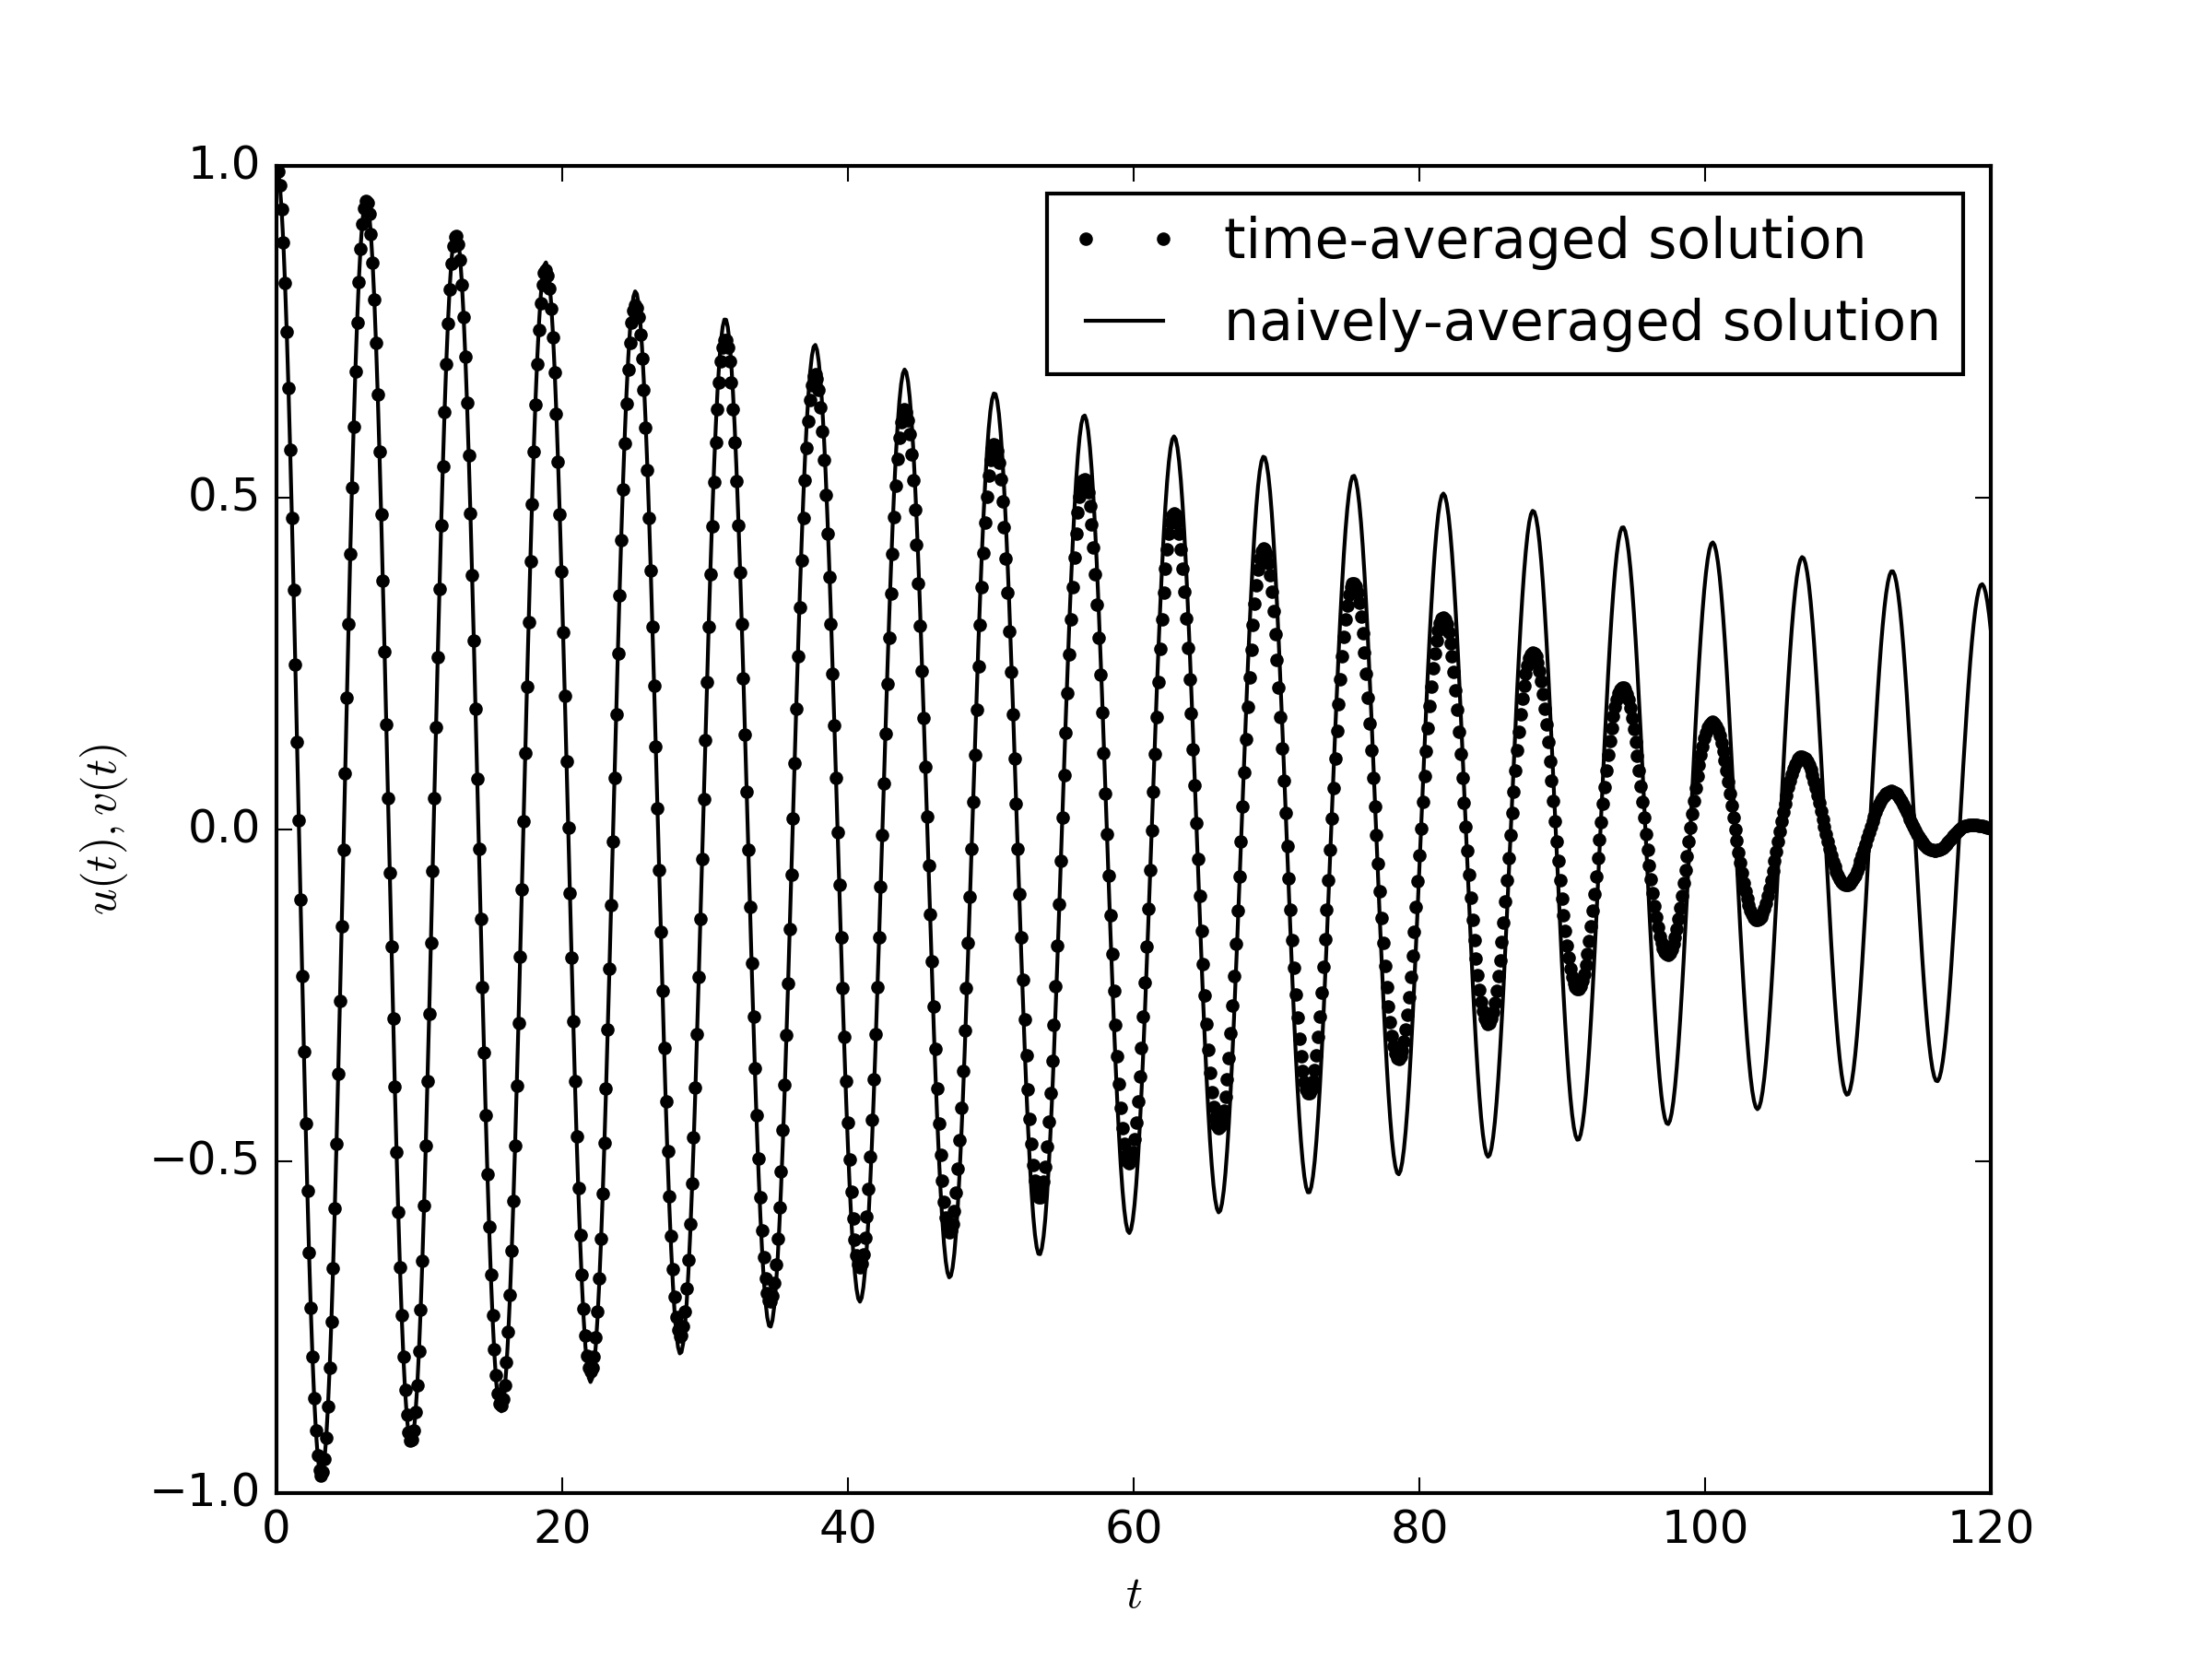
\includegraphics[width=\textwidth]{problem_2.png}
    \end{figure}
\end{proof}






\end{document}
